\documentclass[12pt,a4paper]{article}
\usepackage{ctex}
\usepackage{amsmath,amscd,amsbsy,amssymb,latexsym,url,bm,amsthm}
\usepackage{epsfig,graphicx,subfigure}
\usepackage{enumitem,balance}
\usepackage{wrapfig}
\usepackage{mathrsfs,euscript}
\usepackage[usenames]{xcolor}
\usepackage{hyperref}
\usepackage[vlined,ruled,linesnumbered]{algorithm2e}
\usepackage{array}
\hypersetup{colorlinks=true,linkcolor=black}

\newtheorem{theorem}{Theorem}
\newtheorem{lemma}[theorem]{Lemma}
\newtheorem{proposition}[theorem]{Proposition}
\newtheorem{corollary}[theorem]{Corollary}
\newtheorem{exercise}{Exercise}
\newtheorem*{solution}{Solution}
\newtheorem{definition}{Definition}
\theoremstyle{definition}

\renewcommand{\thefootnote}{\fnsymbol{footnote}}

\newcommand{\postscript}[2]
 {\setlength{\epsfxsize}{#2\hsize}
  \centerline{\epsfbox{#1}}}

\renewcommand{\baselinestretch}{1.0}

\setlength{\oddsidemargin}{-0.365in}
\setlength{\evensidemargin}{-0.365in}
\setlength{\topmargin}{-0.3in}
\setlength{\headheight}{0in}
\setlength{\headsep}{0in}
\setlength{\textheight}{10.1in}
\setlength{\textwidth}{7in}
\makeatletter \renewenvironment{proof}[1][Proof] {\par\pushQED{\qed}\normalfont\topsep6\p@\@plus6\p@\relax\trivlist\item[\hskip\labelsep\bfseries#1\@addpunct{.}]\ignorespaces}{\popQED\endtrivlist\@endpefalse} \makeatother
\makeatletter
\renewenvironment{solution}[1][Solution] {\par\pushQED{\qed}\normalfont\topsep6\p@\@plus6\p@\relax\trivlist\item[\hskip\labelsep\bfseries#1\@addpunct{.}]\ignorespaces}{\popQED\endtrivlist\@endpefalse} \makeatother

\begin{document}
\noindent

%========================================================================
\noindent\framebox[\linewidth]{\shortstack[c]{
\Large{\textbf{Lab07-Amortized Analysis}}\vspace{1mm}\\
CS214-Algorithm and Complexity, Xiaofeng Gao, Spring 2020.}}
\begin{center}
\footnotesize{\color{red}$*$ If there is any problem, please contact TA Shuodian Yu. }

\footnotesize{\color{blue}$*$ Name:Yijia Diao  \quad Student ID:518030910146 \quad Email: diao\_yijia@sjtu.edu.cn}
\end{center}
\begin{enumerate}
	\item For the TABLE-DELETE Operation in Dynamic Tables, suppose we construct a table by multiplying its size by $\frac 23$ when the load factor drops below $\frac 13$. Using \emph{Potential Method} to prove that the amortized cost of a TABLE-DELETE that uses this strategy is bounded above by a constant.
	\begin{proof}
		Assume the potential function:\\
		\begin{align*}
			\Phi(T) = 
			\begin{cases}
			&2\times num[T] - size[T] ,\quad\alpha(T)\ge \frac{1}{2}\\
			&\frac{1}{2}size[T] - num[T],\quad\quad\alpha(T)< \frac{1}{2}
			\end{cases}
		\end{align*}
		\begin{enumerate}
			\item[(1)] $\frac{1}{3}\le\alpha_i \le \frac{1}{2}$, which indicates that the contraction is not triggered. We have
			\begin{align*}
				\widehat{C}_i &= C_i + \Phi_i - \Phi_{i - 1}\\
							  &= 1 + (\frac{1}{2}size_i - num_i) - (\frac{1}{2}size_{i - 1} - num_{i - 1})\\
							  &= 1 + (\frac{1}{2}size_{i - 1} - (num_{i - 1} - 1)) - (\frac{1}{2}size_{i - 1} - num_{i - 1})\\
							  &= 2
			\end{align*}
			\item[(2)] A contraction is triggered, which means $ \alpha_{i}< \frac{1}{2} $. We have
			\begin{align*}
				\widehat{C}_i &= C_i + \Phi_i - \Phi_{i - 1}\\
							  &= num_{i} + 1 + (\frac{1}{2}size_i - num_i) - (\frac{1}{2}size_{i - 1} - num_{i - 1})\\
							  &= num_{i} + 1 + (\frac{1}{2}size_i - num_i) - (\frac{3}{2}size_{i} - num_{i} - 1)\\
							  &= 2 + num_{i} - \frac{1}{2}size_i\\
							  &= 2
			\end{align*}
			\item[(3)] $\alpha_i > \frac{1}{2}$, which indicates that the contraction is not triggered. We have
			\begin{align*}
			\widehat{C}_i &= C_i + \Phi_i - \Phi_{i - 1}\\
			&= 1 + (2\times num_{i} - size_{i}) - (2\times num_{i - 1} - size_{i - 1})\\
			&= 1 + (2\times num_{i - 1} - 1 - size_{i - 1}) - (2\times num_{i - 1} - size_{i - 1})\\
			&= 0
			\end{align*}
		\end{enumerate}
			Therefore,  we can conclude that the amortized cost of a TABLE-DELETE that uses this strategy is bounded above by a constant.
	\end{proof}
	
	\item A \textbf{multistack} consists of an infinite series of stacks $S_0, S_1, S_2,\cdots$, where the $i^{th}$ stack $S_i$ can hold up to $3^i$ elements. Whenever a user attempts to push an element onto any full stack $S_i$, we first pop all the elements off $S_i$ and push them onto stack $S_{i+1}$ to make room. (Thus, if $S_{i+1}$ is already full, we first recursively move all its members to $S_{i+2}$ .) An illustrative example is shown in Figure \ref{Fig-MultiStack}. Moving a single element from one stack to the next takes $O(1)$ time. If we push a new element, \underline{we always intend to push it in stack $S_0$}.

	\begin{figure}[!htbp]
	\centering
	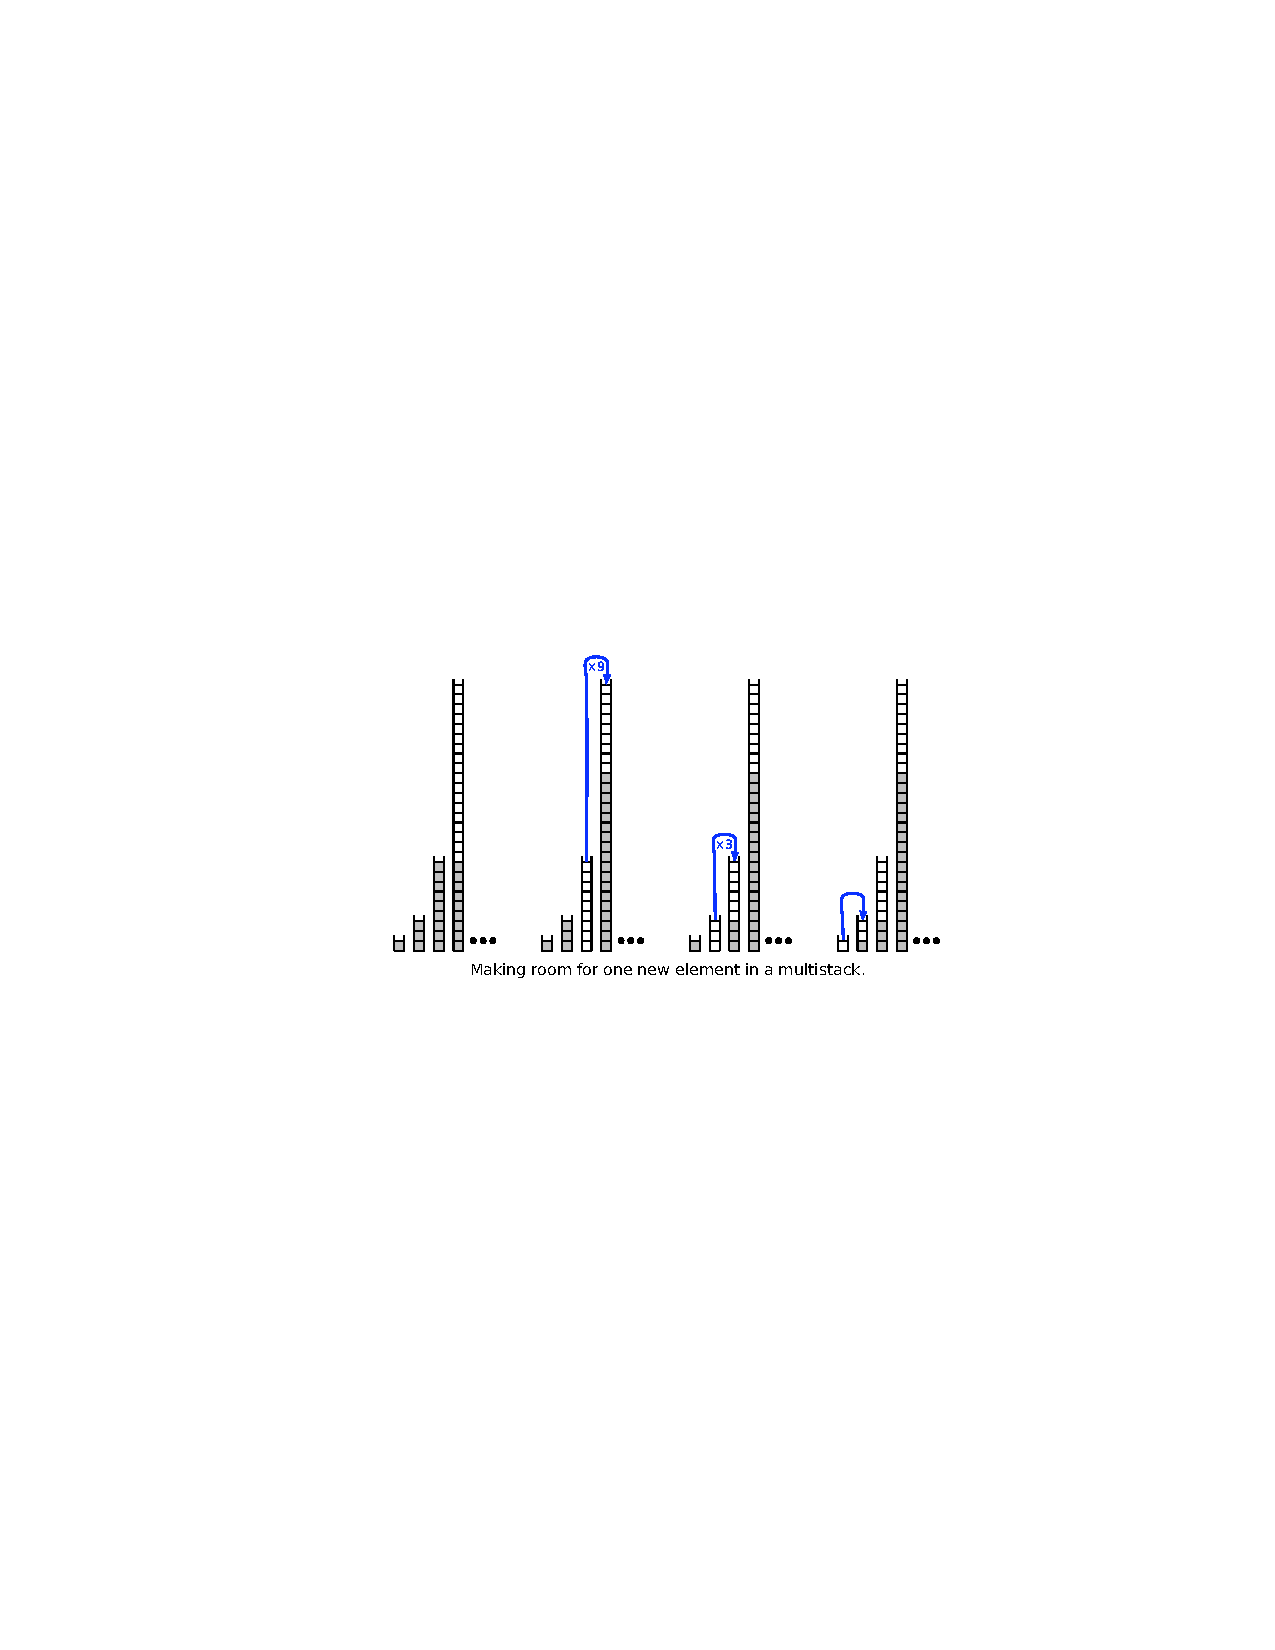
\includegraphics[width=0.5\textwidth]{Fig-MultiStack.pdf}
	\caption{An example of making room for one new element in a multistack.}
	\label{Fig-MultiStack}
	\end{figure}

    \begin{enumerate}
        \item In the worst case, how long does it take to push a new element onto a multistack containing $n$ elements?
        \item Prove that the amortized cost of a push operation is $O(\log n)$ by \emph{Aggregation Analysis}.
        \item {\color{red}(Optional Subquestion with Bonus)} Prove that the amortized cost of a push operation is $O(\log n)$ by \emph{Potential Method}.
    \end{enumerate}

	\begin{solution}
		\begin{enumerate}
			\item The worst case is, when $n=1+\sum_{i=0}^{k}3^i$, all non-empty stacks are already full. Each element needs to be popped and pushed into its next stack, and it takes $T(n)=n$.
			\item 
			Assume the total time of inserting $n$ elements by $S_n$. This is no worse than the case: $n^{th}$ insert is the worst case, which equals to $n=1+\sum_{i=0}^{k}3^i$. So we have
			\begin{align}\label{2b1}
			S_n\leq 1 + 1\times 3^0+2\times 3^1 + \cdots + (k+1)\times 3^k \overset{def}{=} T_k
			\end{align}
			Since
			\begin{align}\label{2b2}
				3\times T_k=3+1\times 3^1+2\times 3^2+\cdots+(k+1)\times 3^{k+1}
			\end{align}
			(Equ.\ref{2b2}$-$Equ.\ref{2b1})$ /2 $, we have
			\begin{align}\label{2b3}
				T_k = \frac{(2k+1)*3^{k+1}+5}{4}
			\end{align}
			Since 
			\begin{align}\label{2b4}
				n\leq 1+(1+3+3^2+\dots+3^k)=\frac{3^{k+1}+1}{2}
			\end{align} 
			From inEqu.\ref{2b3} and inEqu.\ref{2b4}, we have $k<\log_3(2n-1)\le k+1$, which means $ O(k) = O(\log n) $. \\Thus, the amortized cost of a push operation is
			\begin{align*}
			\frac{S_n}{n}\le \frac{T_k}{n}&= \frac{6k+3}{4}\times\frac{2n-1}{n}+\frac{5}{4n}\\
			&=O(k)\\
			&= O(\log n)
			\end{align*}
			$$$$
			\item First assume \textbf{weight function}: $ weight_i = \sum_{j=1}^{k_i}j\times|S_j| $, in which $ k_i $ is the number of non-empty stack after the $i$th insertion. Since $ |S_j| < \log n $, we have $weight_i\leq k_i\log n$. Also, we have $c_i = weight_i - weight_{i-1}$. \\
			Then assume the potential function: 
			$$
			\Phi(i)=\begin{cases}
			k_i\log n- weight_i\nonumber,\quad i>0\\
			0,\quad\quad\quad\quad\quad\quad\quad\quad i=0
			\end{cases}
			$$
			Since $weight_i\leq k_i\log n$, we have $ \forall i >0: \Phi(i)\geq 0\Rightarrow\Phi(n)\geq\Phi(0)$.
			Thus,
			\begin{align*}
				\hat{C_i} &= C_i + \Phi_i - \Phi_{i - 1}\\
					      &= C_i + (k_i\log n- weight_i) - (k_{i-1}\log n- weight_{i - 1})\\
					      &= C_i - (weight_{i} - weight_{i - 1}) + (k_{i} - k_{i - 1})\log n
			\end{align*}
			Since the times of push and pops are $weight_i-weight_{i-1}$, we have
			\begin{align*}
			\hat{C_i} =  (k_{i} - k_{i - 1})\log n = O(\log n)
			\end{align*}
			Therefore, we can conclude that the amortized cost of a push operation is $O(\log n)$.
		\end{enumerate}
	\end{solution}
	
	\item Given a graph $G = (V, E)$, and let $V'$ be a strict subset of $V$. Prove the following propositions.
	
	\begin{enumerate}
		\item Let $T$ be a minimum spanning tree of a $G$. Let $T'$ be the subgraph of $T$ induced by $V'$, and let $G'$ be the subgraph of $G$ induced by $V'$. Then $T'$ is a minimum spanning tree of $G'$ if $T'$ is connected.
		\item Let $e$ be a minimum weight edge which connects $V'$ and $V \setminus V'$. There exists a minimum weight spanning tree which contains e.
	\end{enumerate}
	
	\begin{solution}
		\begin{enumerate}
			\item (Proof by Contradiction) Suppose that $ T' $ is not the minimum spanning tree of $ G' $.\\
			Assume the minimum spanning tree of $ G' $ is $ R $. Since $ T' $ is a connected graph, and is the induced subgraph of $ T $ by $ V' $, we have $ R\backslash T'\neq \emptyset $. Then we construct a subgraph of $ G $: $S =  R\cup(T\backslash T') $. Since $ R $ is the minimum spanning tree of $ G' $, and $ T $ is the minimum spanning tree of $ G $, we have $ S $ is the minimum spanning tree of $ G $. But $ R\backslash T'\neq \emptyset \Rightarrow R \nsubseteq T$, which means $ S\neq T $, contradiction.\\
			Therefore we can conclude that $T'$ is a minimum spanning tree.
			\item (Proof by Contradiction) Suppose that any minimum weight spanning tree does not contain $ e $.\\
			\begin{enumerate}
				\item \label{3.2.1}$ |V'|  = 1$ or $ |V\backslash V'| = 1 $: the minimum weight spanning tree must contain $ e' $, which makes connection with the single vertex and the other part. Suppose the weight of $ \forall e \in G\text{ : } w(e)$, then we have $ w(e) < w(e') $. So if we change $ e' $ to $ e $,  we will get another spanning tree that has a smaller weight. Contradiction.
				\item $ |V'|> 1$ and $ |V\backslash V'| > 1 $: According to this hypothesis, we can find $ V_1\subsetneq V'$, and the minimum spanning tree of $ V' $ does not contain the minimum weight edge between $ V_1$ and $ V'\backslash V_1 $. We can do this division to case \ref{3.2.1}, and it's the same for $ V\backslash V' $. So we still get the contradiction.
			\end{enumerate} 
			Therefore, we can conclude that there exists a minimum weight spanning tree which contains $ e $.
		\end{enumerate}
	\end{solution}
\end{enumerate}



\textbf{Remark:} Please include your .pdf, .tex files for uploading with standard file names.


%========================================================================
\end{document}
